\documentclass[tikz,border=5pt]{standalone}
\usepackage{tikz}
\usetikzlibrary{arrows.meta}
\definecolor{nebula}{HTML}{6366F1}
\definecolor{spark}{HTML}{14B8A6}
\definecolor{ink}{HTML}{334155}
\begin{document}
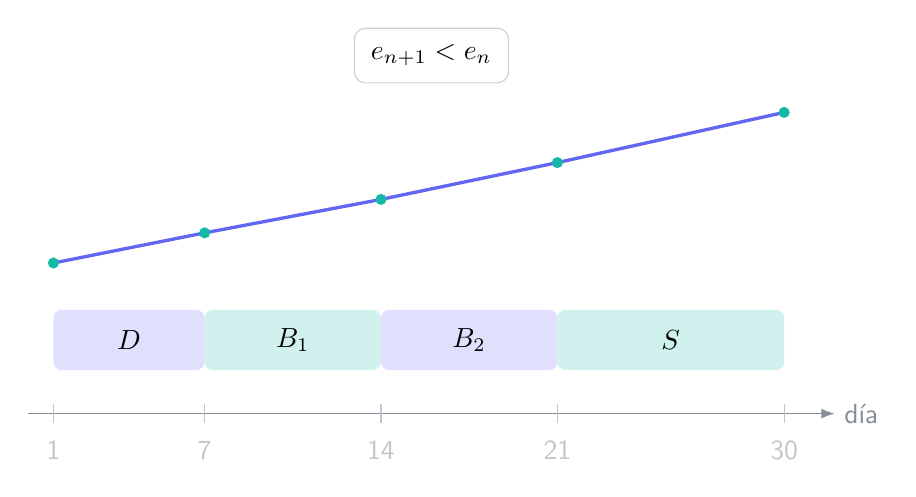
\begin{tikzpicture}[font=\sffamily,>=Latex,x=.32cm,y=.85cm]
  \draw[->,ink!60] (0,0)--(32,0) node[right] {día};
  \foreach \x in {1,7,14,21,30}{\draw[ink!30] (\x,.14)--(\x,-.14) node[below=3pt] {\x};}
  \fill[nebula!20,rounded corners=3pt] (1,.65) rectangle (7,1.55);
  \fill[spark!20,rounded corners=3pt] (7,.65) rectangle (14,1.55);
  \fill[nebula!20,rounded corners=3pt] (14,.65) rectangle (21,1.55);
  \fill[spark!20,rounded corners=3pt] (21,.65) rectangle (30,1.55);
  \node at (4,1.1) {$D$}; \node at (10.5,1.1) {$B_1$}; \node at (17.5,1.1) {$B_2$}; \node at (25.5,1.1) {$S$};
  \draw[very thick,nebula] (1,2.25)--(7,2.7)--(14,3.2)--(21,3.75)--(30,4.5);
  \foreach \p in {(1,2.25),(7,2.7),(14,3.2),(21,3.75),(30,4.5)}{\fill[spark] \p circle (2pt);}
  \node[draw=ink!25,rounded corners=4pt,fill=white,inner sep=6pt] at (16,5.35)
    {$e_{n+1}<e_n$};
\end{tikzpicture}
\end{document}
